\documentclass{beamer}

\sloppy

\usepackage[T2A]{fontenc}
\usepackage[utf8x]{inputenc}

\usepackage[english,russian]{babel}

\usepackage{cite}

\usepackage{changepage}
\usepackage{pdflscape}

\usepackage{float}

\EqInChapter
\TableInChapter
\PicInChapter

\usepackage[
bookmarks=true, colorlinks=true, unicode=true,
urlcolor=black,linkcolor=black, anchorcolor=black,
citecolor=black, menucolor=black, filecolor=black
]{hyperref}

\usepackage{graphicx}
\graphicspath{{..//images/}}

\newcommand{\Code}[1]{\textbf{#1}}

\geometry{right=10mm}
\geometry{left=25mm}


\begin{document}
\frame{\titlepage}

\frame{
  \frametitle{Актуальность}
  \begin{itemize}
    \item Ключевая фраза (англ. \emph{keyphrase}) —
выражение, состоящее из одного или нескольких ключевых слов,
представляющее собой важнейший информационный сегмент документа.
  \end{itemize}
  Сегодня интеллектуальные информационные системы нашли широкое
применение в области здравоохранения.
  \begin{itemize}
    \item Одной из важнейших составляющих современных медицинских
информационных систем является подсистема интеллектуального анализа
текстовых данных.
    \item Адекватность функционирования подсистемы интеллектуального
анализа текстовых данных напрямую зависит от качества работы модуля
извлечения ключевых фраз.
  \end{itemize}
}

\frame{
  \frametitle{Задача выделения ключевых слов и фраз}
  В общем виде, задача возникает в библиотечном деле,
лексикографии и терминоведении, а также в информационном поиске.
  \begin{itemize}
    \item Ключевые фразы могут использоваться для создания и
развития терминологических ресурсов, а также для эффективной
обработки документов: индексирования, реферирования, классификации и
визуализации.
  \end{itemize}
}

\frame{
  \frametitle{Системы автоматического извлечения ключевых фраз}
  Существующие системы:
  \begin{itemize}
    \item разработаны на Западе и ориентированы исключительно на
обработку западноевропейских языков;
    \item разработаны в России и непригодны для использования
из-за устаревших и неэффективных методов извлечения ключевых фраз,
а также ограничительных условий распространения.
  \end{itemize}
}

\frame{
  \frametitle{Аналоги}
  Существует большое количество систем автоматического извлечения
ключевых фраз из текста на естественном языке:
  \begin{itemize}
    \item OpenCalais.
    \item Extractor.
    \item Yahoo! Term Extraction Service.
    \item TerMine.
    \item Maui.
    \item TextAnalyst.
    \item AOT.
    \item ContentAnalyzer.
    \item Семантическое зеркало.
  \end{itemize}
}

\frame{
  \frametitle{Критерии оценки аналогов}
  Необходимая система автоматического извлечения ключевых фраз из
текста на естественном языке оценивается по следующим практически
важным критериям:
  \begin{itemize}
    \item поддержка русского языка (``Р'');
    \item качество результата по итогам экспертной оценки (``К'');
    \item доступность аналога (``Д'');
    \item независимость аналога от наличия онтологии заданной
области знаний или специализированного тезауруса в процессе
извлечения ключевых фраз (``О'').
  \end{itemize}
}

\frame{
  \frametitle{Сравнение аналогов}
  \begin{table}
  \begin{center}
  \begin{tabular}{|c||c||*{4}{p{7mm}|}|c|}
\hline
  & Название & \multicolumn{4}{c||}{Оценки по критериям} & \\
                \cline{3-6}
№ & аналога         &  Р  &  К  &  Д  &  О  & \huge $\Sigma$ \\
\hline
\hline
1 & OpenCalais      & 0.0 & 0.8 & 0.5 & 0.0 & 1.3 \\
\hline
2 & Extractor       & 0.0 & 0.7 & 0.0 & 1.0 & 1.7 \\
\hline
3 & Yahoo!~T.E.W.S. & 0.0 & 0.6 & 0.5 & 1.0 & 2.1 \\
\hline
4 & TerMine         & 0.0 & 0.7 & 0.5 & 1.0 & 2.2 \\
\hline
5 & Maui            & 0.0 & 0.6 & 1.0 & 1.0 & 2.6 \\
\hline
6 & TextAnalyst     & 1.0 & 0.3 & 0.5 & 1.0 & 2.8 \\
\hline
\textbf{7} & \textbf{AOT}
                    & 1.0 & 0.4 & 1.0 & 1.0 & \textbf{3.4} \\
\hline
8 & ContentAnalyzer & 1.0 & 0.6 & 0.5 & 1.0 & 3.1 \\
\hline
9 & Сем.~зеркало    & 1.0 & 0.5 & 0.5 & 1.0 & 3.0 \\
\hline
  \end{tabular}
  \end{center}
  \end{table}
Целесообразным является выбор аналога №7 (\textbf{AOT}) в качестве
прототипа системы автоматического извлечения ключевых фраз из
текста на естественном языке.
}

\frame{
  \frametitle{Структурная модель прототипа}
  \begin{figure}
    \centering
    \subfloat{\includegraphics[height=.75\textheight]{Prototype.eps}}
  \end{figure}
}

\frame{
  \frametitle{Описание схемы функционирования прототипа}
  \begin{figure}
    \centering
    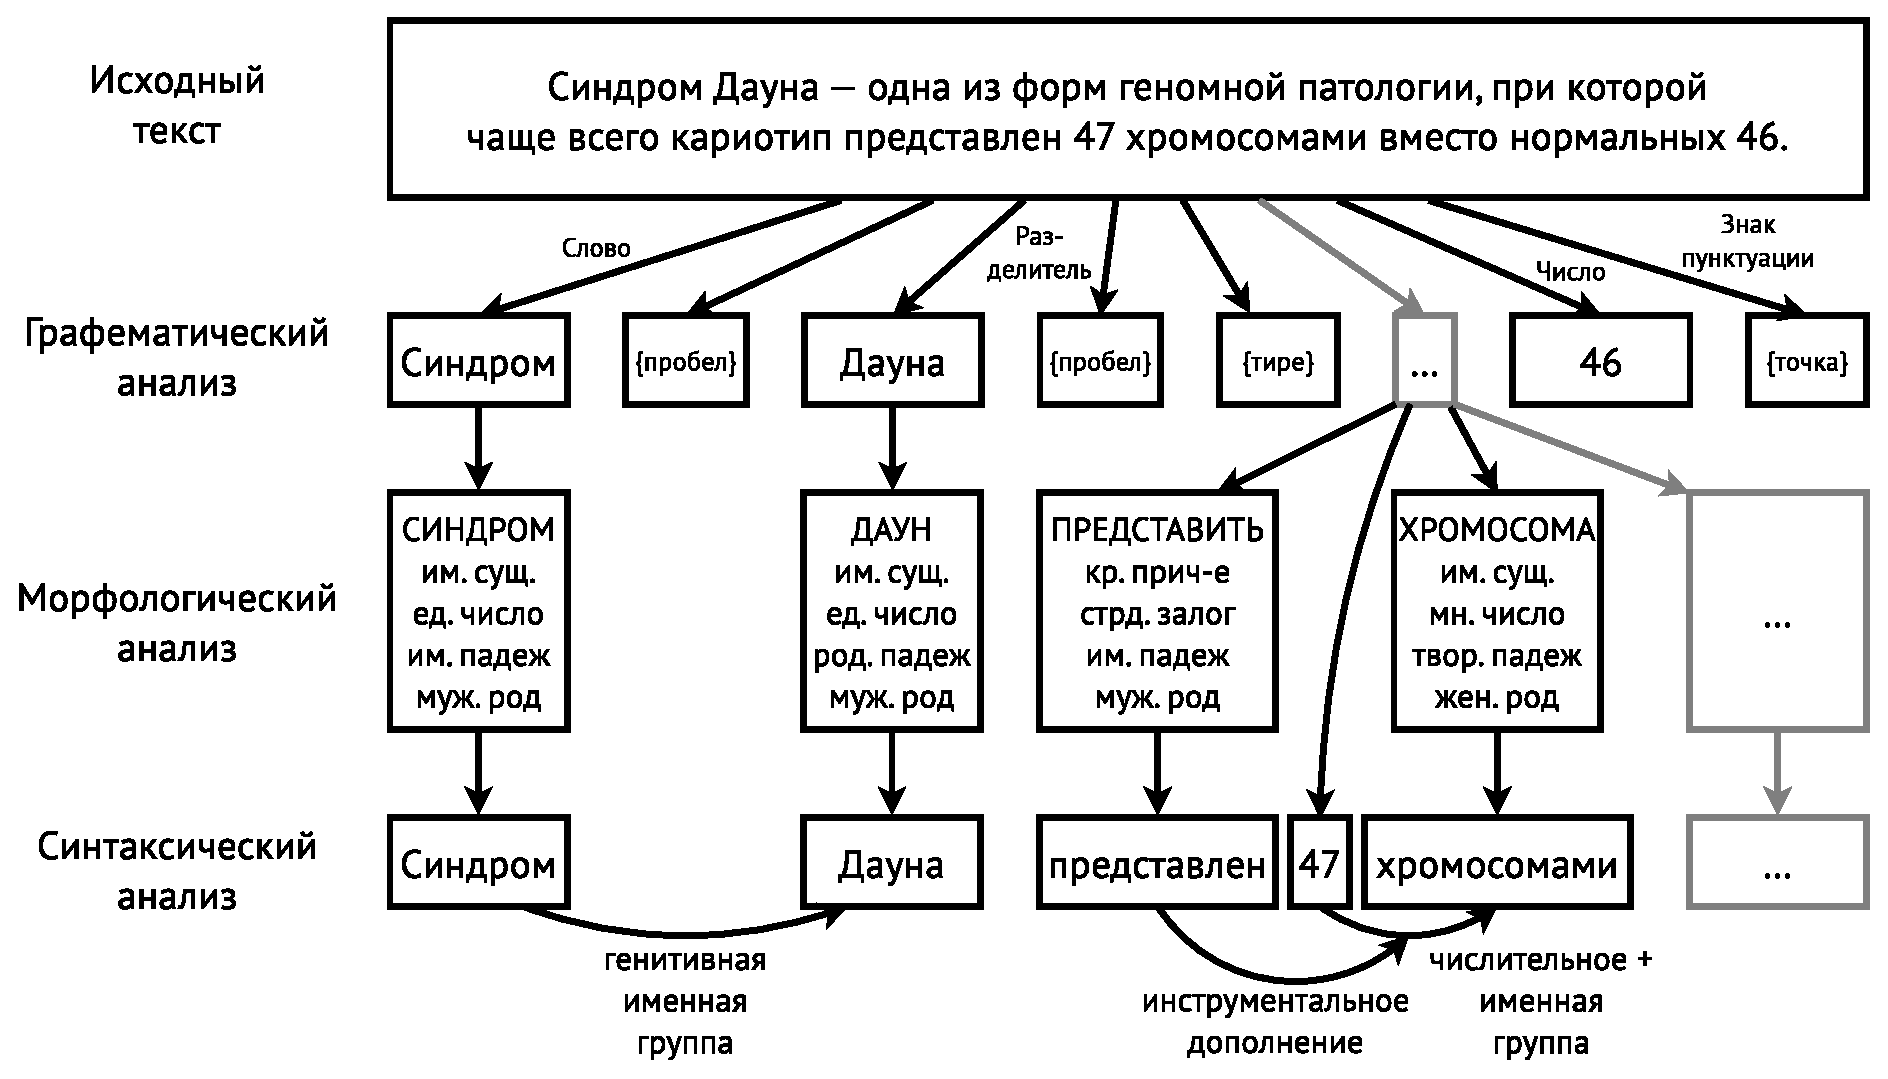
\includegraphics[width=\textwidth]{Example.eps}
  \end{figure}
}

\frame{
  \frametitle{Критика прототипа}
  Критический анализ:
  \begin{itemize}
    \item применённый в прототипе метод распознавания ключевых фраз
обладает недостаточной точностью;
    \item стоит отметить, что качество работы современных
морфологических анализаторов превосходит морфологический анализатор
АОТ.
  \end{itemize}
}

\frame{
  \frametitle{Предлагаемое решение}
  Меры по развитию прототипа:
  \begin{itemize}
    \item внести в структуру прототипа блок, вычисляющий
статистическое значение терминологичности каждой именной группы,
выделенной синтаксическим анализатором;
    \item необходимо модифицировать морфологический анализатор
системы АОТ, что повысит качество предварительной обработки текста и
положительно скажется на результате работы всей системы в целом.
  \end{itemize}
}

\frame{
  \frametitle{Метрика C-value}
  Предлагается вычислять значение терминологичности при помощи
статистической метрики C-value по формуле:
\begin{equation*}
  C-value(a) = \begin{cases}
    log_{2}|a| \cdot f(a), &
                 \mbox{если } a \mbox{ не вложен} \\
    log_{2}|a| \cdot f(a) - \frac{1}{P(T_{a})}
               \cdot \sum_{b \in T_{a}} f(b), &
                 \mbox{если } a \mbox{ вложен},
  \end{cases}
\end{equation*}
где $a$ — кандидат в термины; \\
$|a|$ — длина словосочетания, измеряемая в количестве слов; \\
$f(a)$ — частотность $a$; \\
$T_{a}$ — множество словосочетаний, которые содержат $a$; \\
$P(T_{a})$ — количество словосочетаний, содержащих $a$.
  \begin{itemize}
    \item \small Аналогичное решение применено в системе TerMine,
получившей наивысшую оценку качества результата работы среди систем,
не использующих онтологию заданной области знаний в процессе
выделения ключевых фраз.
  \end{itemize}
}

\frame{
  \frametitle{Структурная модель блока выделения ключевых фраз}
  \begin{figure}
    \centering
    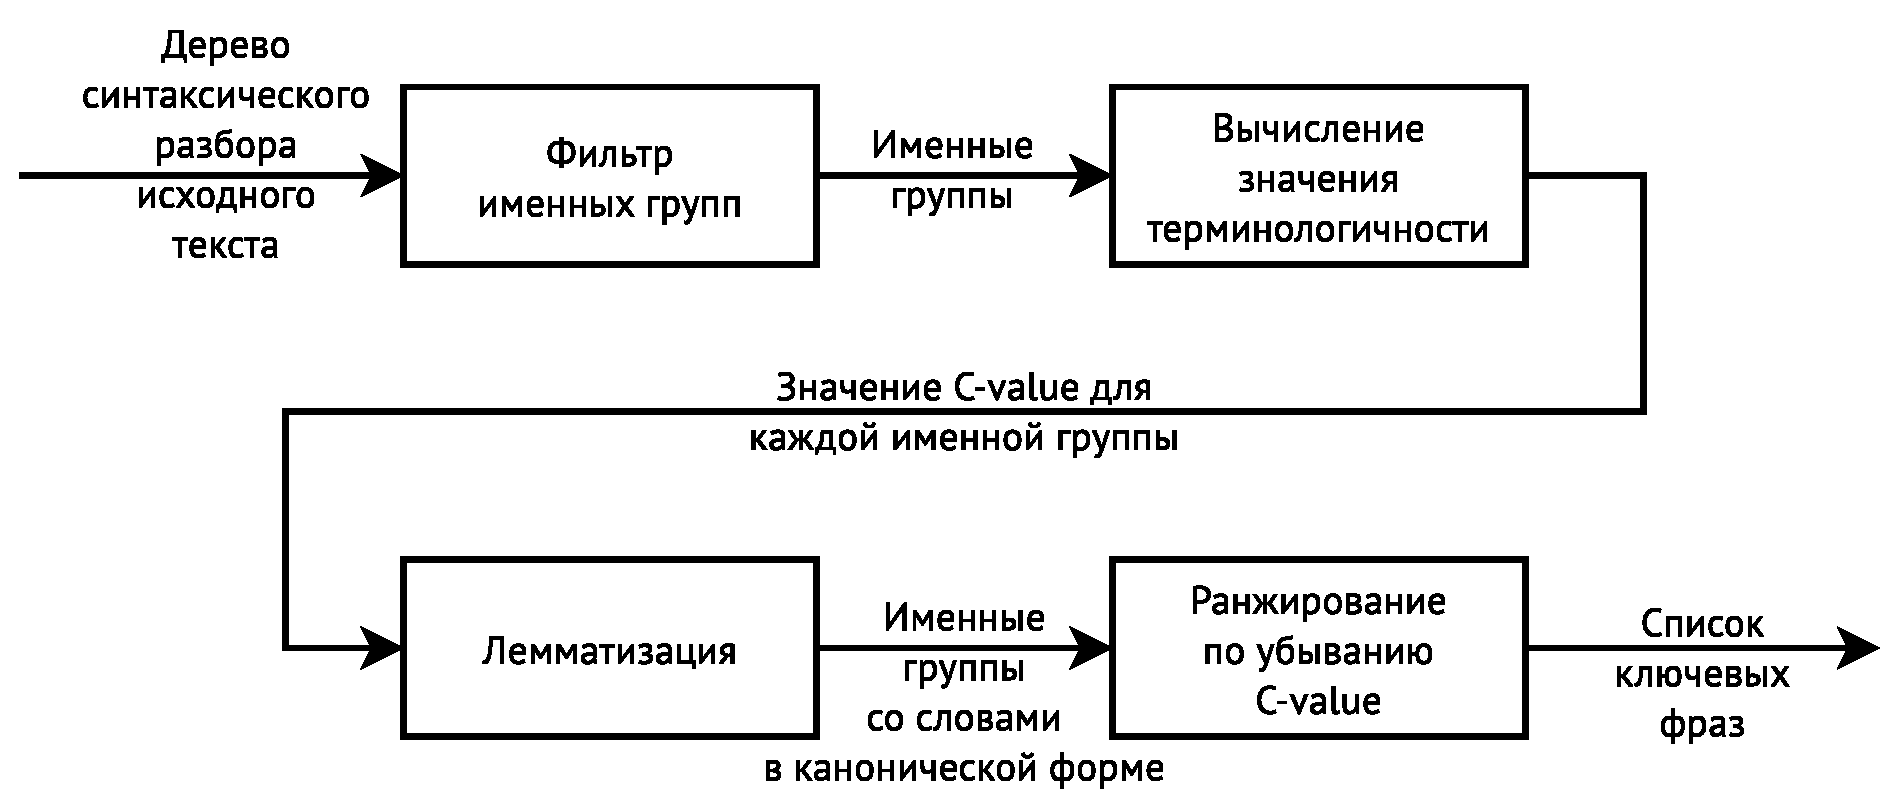
\includegraphics[width=\textheight]{Solution-Rank1a.eps}
  \end{figure}
}

\frame{
  \frametitle{Критерии оценки морфологического анализатора}
  В качестве критериев сравнения морфологических анализаторов
выберем:
  \begin{itemize}
    \item поддержка русского языка (``Р'');
    \item возможность определения части речи и грамматических
характеристик слова (``Ч'');
    \item возможность выделения основы слова (``О'');
    \item качество анализа по итогам экспертной оценки (``К'');
    \item доступность аналога (``Д'').
  \end{itemize}
}

\frame{
  \frametitle{Сравнение морфологических анализаторов}
  \begin{table}
  \begin{center}
  \begin{tabular}{|c||c||*{5}{p{5mm}|}|c|}
\hline
  & Название   & \multicolumn{5}{c||}{Оценки по критериям} & \\
                \cline{3-7}
№ & аналога    &  Р  &  Ч  &  О  &  К  &  Д  & \huge $\Sigma$ \\
\hline
\hline
1 & АОТ        & 1.0 & 1.0 & 1.0 & 0.6 & 1.0 & 4.6 \\
\hline
2 & mystem     & 1.0 & 1.0 & 1.0 & 0.8 & 0.5 & 4.3 \\
\hline
3 & Snowball   & 1.0 & 0.0 & 1.0 & 0.6 & 1.0 & 3.6 \\
\hline
\textbf{4}
  & \textbf{myaso}
               & 1.0 & 1.0 & 1.0 & 0.7 & 1.0 & \textbf{4.7} \\
\hline
5 & pymorphy   & 1.0 & 1.0 & 1.0 & 0.5 & 1.0 & 4.5 \\
\hline
6 & TreeTagger & 1.0 & 1.0 & 1.0 & 0.7 & 0.5 & 4.2 \\
\hline
7 & TnT        & 1.0 & 1.0 & 0.0 & 0.7 & 0.5 & 3.2 \\
\hline
  \end{tabular}
  \end{center}
  \end{table}
Целесообразным является выбор аналога №4 (\textbf{myaso}) в качестве
готового морфологического анализатора.
}

\frame{
  \frametitle{Структурная модель предлагаемого решения}
  \begin{figure}
    \centering
    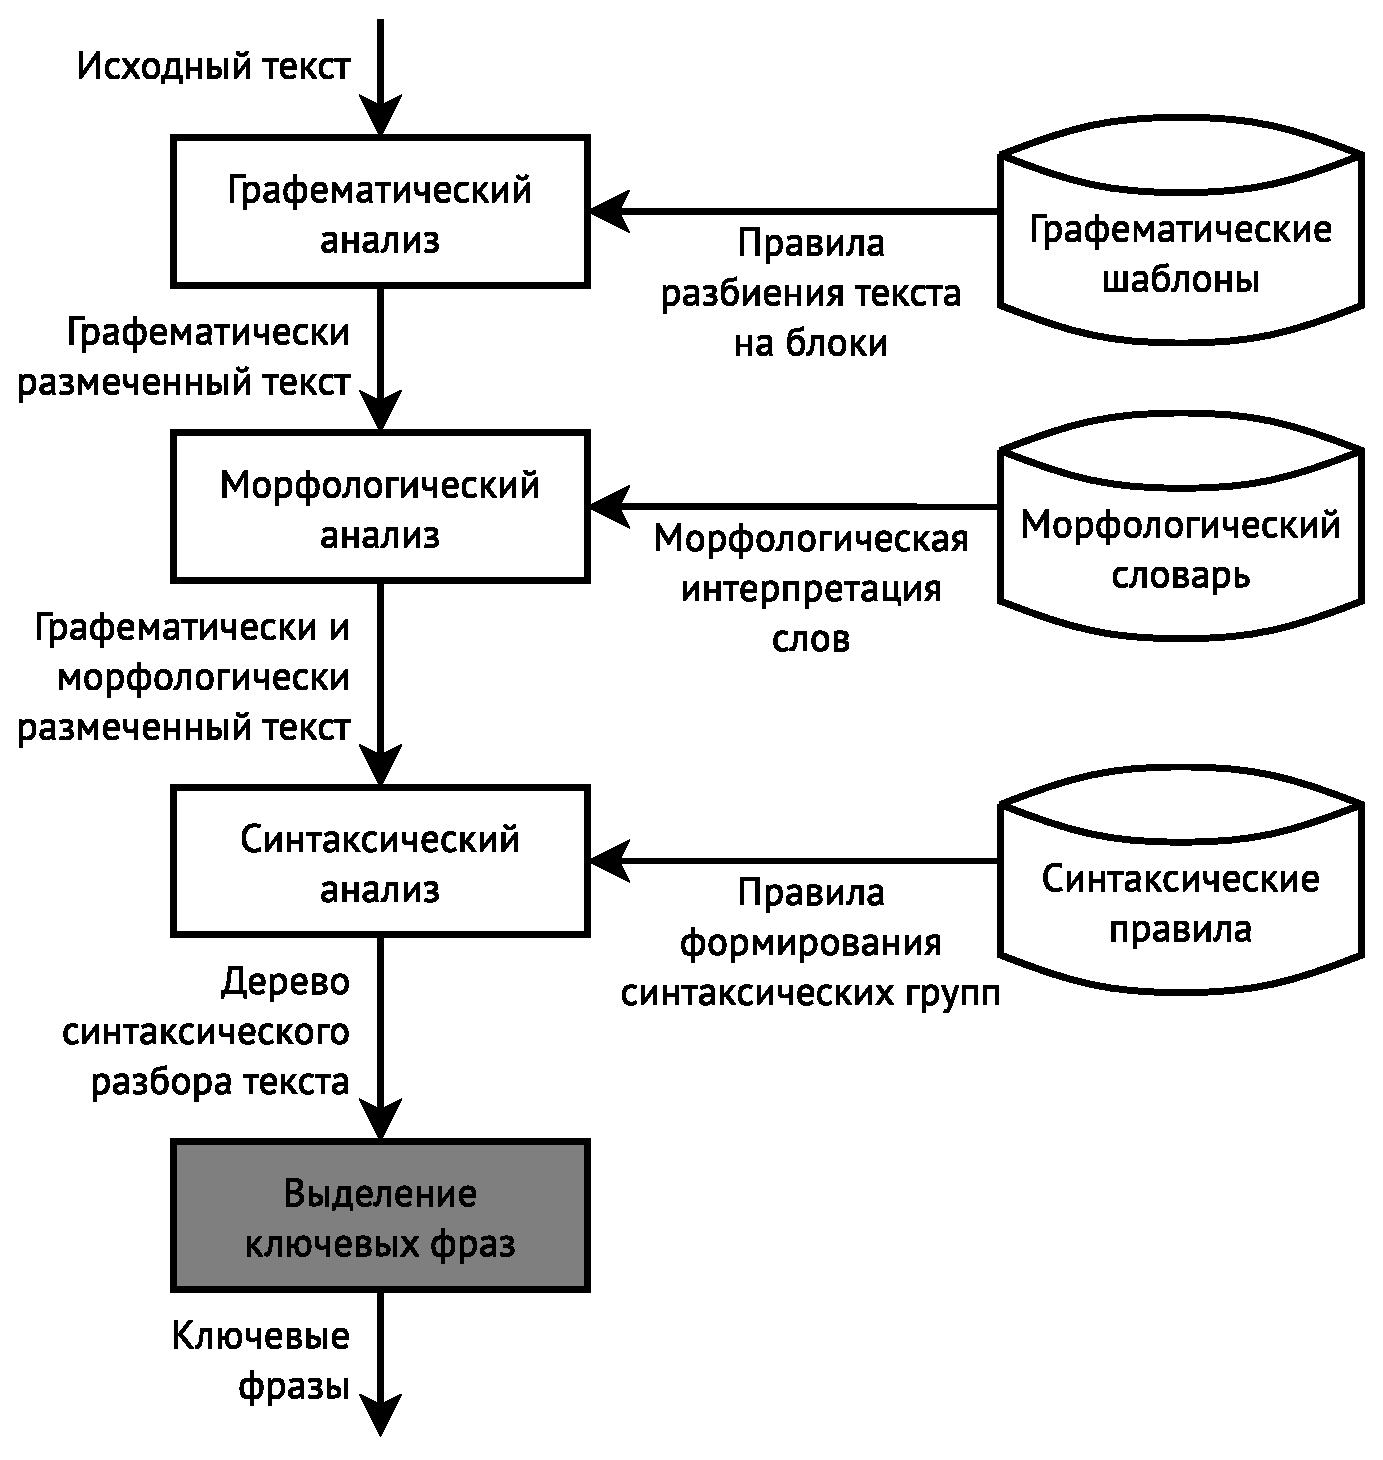
\includegraphics[height=.75\textheight]{Solution-Rank0.eps}
  \end{figure}
}

\frame{
  \frametitle{Проектирование решения}
  В результате проектирования предлагаемого решения разработано
Техническое задание, которое приведено в приложении Б:
  \begin{itemize}
    \item для разработки выбрана платформа Rubinius —
перспективная реализация языка программирования Ruby на основе
виртуальной машины LLVM;
    \item система построена на основе архитектуры REST и стандартных
протоколов JSON и XML;
    \item предусмотрена возможность запуска системы в «облачной»
среде.
  \end{itemize}
}

\frame{
  \frametitle{Главная страница Web-интерфейса}
  \begin{figure}
    \centering
    \includegraphics[width=\textwidth]{Tesuck-Index.png}
  \end{figure}
}

\frame{
  \frametitle{Страница результатов работы Web-интерфейса}
  \begin{figure}
    \centering
    \includegraphics[height=.75\textheight]{Tesuck-Result.png}
  \end{figure}
}

\frame{
  \frametitle{Вклад в свободное программное обеспечение}
  Система Tesuçk полностью построена на основе свободного
программного обеспечения. В процессе инженерной реализации возникла
необходимость доработки существующих решений:
  \begin{itemize}
    \item sinatra/config-file;
    \item ffi-rzmq.
  \end{itemize}
  Все внесённые изменения поддержаны авторами оригинальных продуктов
и востребованы сообществом.
}

\frame{
  \frametitle{Внедрение}
  На сегодняшний день достигнуты следующие результаты:
  \begin{itemize}
    \item система Tesuçk развёрнута в PaaS-облаке Cloud Foundry,
расположенном в ЦОД ИММ УрО РАН и доступна широкой публике по URL:
\url{http://tesuck.eveel.ru};
    \item ведутся работы по интеграции Tesuçk в популярный сервис
коллективных переводов \url{http://translated.by} по договорённости
с компанией JetStyle.
  \end{itemize}
}

\frame{
  \frametitle{Дальнейшая работа}
  Направления дальнейшей работы:
  \begin{itemize}
    \item выступление и презентация работы на RuSSIR/EDBT 2011;
    \item оформление интеллектуальной собственности;
    \item магистерская диссертация: построить систему синтеза
изображения по тексту на основе Tesuçk.
  \end{itemize}
  \begin{figure}
    \centering
    \includegraphics[height=.5\textheight]{Ponies/Pinkie-Pie.jpg}
  \end{figure}
}

\frame{
  \frametitle{У меня всё}
  \begin{center}
    Спасибо за внимание!
    \begin{figure}
      \includegraphics[height=.6\textheight]{Ponies/Twilight-Sparkle.jpg}
    \end{figure}
  \end{center}
}

\end{document}
